\chapter{Q-Learning}




\section{Reinforcement Learning}

Reinforcement learning (RL) refers to both a learning problem and a subfield of machine
learning. As a learning problem, it refers to learning to control a system so as to maximize
some numerical value which represents a long-term objective. A typical setting where
reinforcement learning operates is shown in Figure \ref{fig:agentenv}: A controller receives the controlled
system’s state and a reward associated with the last state transition. It then calculates an
action which is sent back to the system.


\begin{figure}
\centering
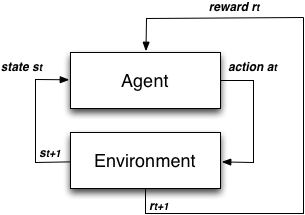
\includegraphics[width=0.7\textwidth]{./images/agentenv.png}
\caption{Example of a simple MDP with three states and two actions}
\label{fig:agentenv}
\end{figure}


The basis idea of Reinforcement learning  is simply to capture the most important aspects of the real problem facing a learning agent interacting with its environment to achieve a goal \cite{Sutton2012}. Reinforcement learning is learning what to do—how to map situations to actions—so as to maximize a numerical reward signal. The learner need to discover which actions yield the most reward by trying them \cite{Sutton2012}.

In Reinforcement Learning, an agent wanders in an unknown environment and tries to maximize its long term return by performing actions and receiving rewards. The challenge is to understand how a current action will affect future rewards. A good way to model this task is with Markov Decision Processes (MDP), which have become the dominant approach in Reinforcement Learning. There are two types of learning problems:

\begin{itemize}
\item Iteractive learning;
\item Non-interactive learning.
\end{itemize}

In non-interactive learning, the natural goal is to find a good policy given a fixed number of observations. A common situation is when the sample is fixed. For example, the sample can be the result of some experimentation with some physical system that happened before learning started. 

In Interactive learning, learning happens while interacting with a real system in a closed-loop fashion. A reasonable goal then is to optimize online performance,
making the learning problem an instance of online learning. Online performance can be measured in different ways. A natural measure is to use the sum of rewards incurred during learning. 

Interactive learning is potentially easier since the learner has the additional option to influence the distribution of the sample. However, the goal of
learning is usually different in the two cases, making these problems incomparable in general.

In Reinforcement Learging, all agents act in two phases: Exploration vs Explotation. In Exploration phase, the agents tries discover better action selections to improve its knowledge. In Explotation phase, the agents tries to maximize its reward, based on what its already know.

One of the challenges that arise in reinforcement learning is the trade-off between exploration and exploitation. To obtain a lot of reward, a reinforcement learning
agent must prefer actions that it has tried in the past and found to be effective in producing reward.
But to discover such actions, it has to try actions that it has not selected before. The agent has to exploit what it already knows in order to obtain reward, but it also has to explore in order to make better action selections in the future.





\subsection{Markov decision processes}

Markov decision processes (MDPs) provide a mathematical framework for modeling decision making. A countable MDP is defined as a triplet $M=(\chi,A,P_{0})$ \cite{Szepesvari2010}. where $\chi$ is a set of states, A is a set of actions. The transition probability kernel $P_{0}$ assigns to each state-action pair $(x, a) \in \chi x A $


The six main elements of a MDP are:(1) state of the system, (2) actions, (3) transition probabilities, (4) transition rewards, (5) a policy, and (6) a performance metric \cite{Sutton2012}.

\begin{figure}
\centering
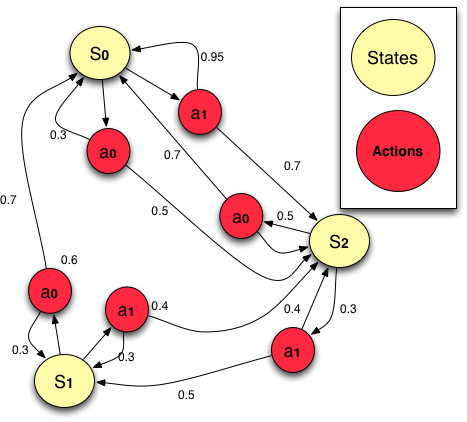
\includegraphics[width=0.7\textwidth]{./images/mdp1.png}
\caption{Example of a simple MDP with three states and two actions}
\label{fig:mdp}
\end{figure}


The state of a system is a parameter or a set of parameters that can be used to describe a system. For example the geographical coordinates of a robot can be used to
describe its state. A system whose state changes with time is called a dynamic system. Then it is not hard to see why a moving robot produces a dynamic system.

Actions are the controls allowed for an agent. Transition Probability denotes the probability of going from state i to state j under the influence of action a in one step. If an MDP has 3 states and 2 actions, there are 9 transition probabilities per action. Usually, the system receives an immediate reward ,which could be positive or negative, when it transitions from one state to another

A policy defines the learning agent’s way of behaving at a given time. Roughly speaking, a policy is a mapping from perceived states of the environment
to actions to be taken when in those states. It corresponds to what in
psychology would be called a set of stimulus–response rules or associations.  Policys mapping from states to actions.

Performance Metric: Associated with any given policy, there exists a so-called performance
metric — with which the performance of the policy is judged. Our goal is to select the policy
that has the best performance metric. 


\section{Q-Learning}

Q-learning is a model-free reinforcement learning technique. Q-learning, it is a multiagent learning algorithm that learns equilibrium policies in Markov games, just as Q-learning learns to optimal policies in Markov decision processes \cite{Greenwald2003}. 

Q-learning and related algorithms tries to learn the optimal policy from its history of interaction with the environment. A history of an agent is a sequence of state-action-rewards.Where $s_{n}$ it is a state, $a_{n}$ it is an action and $r_{n}$ is a reward:

\begin{equation}
<s_{0},a_{0},r_{1},s_{1},a_{1},r_{2},s_{2},a_{2},r_{3},s_{3},a_{3},r_{4},s_{4}....>,
\end{equation}


In Q-Learning, the system's objective is to learn a control policy $\pi = \sum_{n=0}^{\infty} \gamma\textsuperscript{n}  r_{t}+n $, where $\pi$  is the discounted cumulative reward, $\gamma$ is the discount rate ($01$) and $r_{t}$ is the reward reiceved after execution an action at time t. The fig. \ref{fig:qalgo} shows the summary version of Q-Learning algorithm. The first step it is to generate the initial state of the MDP. The second step it is to choose the best action or a random action based on the reward, the actions with best rewards are chosen.


\begin{figure}[h!]
\centering
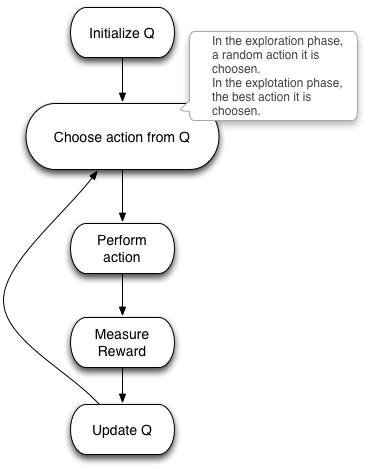
\includegraphics[width=0.8\textwidth]{./images/qalgo.png}
\caption{Q Learning algorithm}
\label{fig:qalgo}
\end{figure}


\section{GridWorld Example}

The GridWorld problem is an example of using reinforcement learning with Q-Learning. In this example,  The agent's goal is to reach the reward state.  There are one rewarding states with value +1 (Gray square at position (3,1)). The agent receives +0.02 of reward if it get closer to the reward state  As the agent moves away from the reward state, he receives -0.01 of reward.The agente receive +0 points of reward if it is the same distance to the reward state.

The Fig. \ref{fig:gridworld} shows the initial and final phase on exploration phase. The numbers in the squares shows the Q-values  for four available actions: up (u), left (l), right(r) and down(d). The arrows show the optimal action based on the current value function. The initial discount rate is 0.9. 

\begin{figure}[h!]
\centering
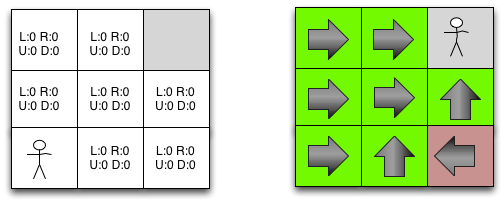
\includegraphics[width=1\textwidth]{./images/mdpgridworld.png}
\caption{GridWorld - initial and final stage on exploration phase}
\label{fig:gridworld}
\end{figure}

The figure  \ref{fig:gridworld1},\ref{fig:gridworld2}, \ref{fig:gridworld3} and \ref{fig:gridworld4}   shows the states of the game in exploration phase. In the first image, all frames have the accumulated reward value equals to zero. In the second image the reward values increase or decrease as the agent moves.

\section{Relationships Between Reinforcement Learning and Optimization}

Many are the intersections between optimization and Reinforcement Learning. First, approximated versions of optimazation and RL tasks contain challenging optimization tasks,  the maximization operations in determining the best action when an action value function is available or the optimal choice of approximation \cite{Battiti2009}. Both optimization and Machine Learning analysts address real world problems by formulating a model, deriving the core optimization problem, and using mathematical programming to solve it \cite{Bennett2006} \cite{Boyan2000}. 

Gambardella et al. show an Ant metaheuristic with Q-Learning approach (Ant-Q). They experimentally investigate the functioning of Ant-Q and we show that the results obtained by Ant-Q on symmetric TSP's are competitive with those obtained by other heuristic approaches based on neural networks or
local search. The research used Q-Learning to indicate how useful it is to make move in TSP for each ant \cite{Gambardella1995}.  Bianchi et at.  present a new algorithm, called Heuristically Accelerated Q–Learning (HAQL), that allows the use of heuristics to speed up the well-known Reinforcement Learning algorithm Q–learnin    g. The Heuristically Accelerated Q–Learning algorithm can be defined as a way of solving the RL problem which makes explicit use of a heuristic function to influence the choice of actions during the learning process. The HAQL uses a modification Greedy rule to control exploration and exploitation phases \cite{Matsuura2015}. 

\section{Software Testing with Reinforcement Learning}

Many software systems are reactive. The behavior of a reactive system, especially when distributed or multithreaded, can be nondeterministic. In these cases, a test suite generated offline may be infeasible.

Online testing is a formal model-based testing (MBT),where the tester uses a specification of the system's behavior to guide the testing and to detect the discrepancies between the aplication under test and the model.Online testing can be more appropriate than offline tests for reactive systems. The reason is that with online testing the tests may be dynamically adapted at runtime, effectively pruning the search space to include only those behaviors actually observed instead of all possible behaviors. The interaction between tester and the application under test is seen as a game  where the tester chooses moves based on the observed behavior of the implementation under test \cite{Havelund2006}.

Havelund et al transforms online testing problem into a special case of reinforcement learning where the frequencies of various abstract behaviors are recorded and allows to better choose controllable actions \cite{Havelund2006}.

Andre et al. show a method that operationalizes the risk assessment for interoperability testing. Typically high number of possible interaction scenarios makes interoperability testing a complex task. Since it seems impossible to cover all scenarios, their relevance for being tested has to be prioritized. The method uses behavior models of the system under test and reinforcement learning techniques to obtain the relevance of single system actions for being tested \cite{Piel2010}. The table \ref{tab:testq1} shows the Q-value for some states of the test. 


% Please add the following required packages to your document preamble:
% \usepackage[table,xcdraw]{xcolor}
% If you use beamer only pass "xcolor=table" option, i.e. \documentclass[xcolor=table]{beamer}
\begin{table}[h]
\centering
\caption{Q-value for some states of the test \cite{Piel2010}}
\label{tab:testq1}
\begin{tabular}{lll}
\rowcolor[HTML]{C0C0C0} 
\textbf{State} & \textbf{Action} & \textbf{Q-value} \\
M'1N1O1       & M 1 → M 2       & 2.5              \\
M'2N2O2       & M 2 → M 1       & 1.25             \\
M'2N2O2       & M 2 → M 3       & 0.0              \\
M'1N1O2       & M 1 → M 2       & 0.5             
\end{tabular}
\end{table}


Sato and Sugihara propose an automatic test pattern generation by applying genetic algorithms in reinforcement learning. The results of evaluation with an ATM system which assuming the existence of a bug related to a global variable are reported \cite{sato2015automatic}. 

Meinke and Niu presents an application of learning techniques to the problem of automated test case generation for numerical software. Our approach uses n-dimensional polynomial models as an algorithmically learned abstraction of the application under test. Test cases are iteratively generated by applying a satisfiability algorithm to first-order program specifications over real closed fields and iteratively refined piecewise polynomial models \cite{Meinke2010}. Kamali et al. propose a  approach based on Q-learning, on top of genetic algorithms (GA) to determine the best weightings for an metaheuristic \cite{Kamali2007}.

